\section*{Spécifications matérielles}

\begin{table}

\label{my-label}

\begin{tabular}{l|p{90mm}}
\hline
\rowcolor[HTML]{FFFFFF} 
\multicolumn{2}{c}{\cellcolor[HTML]{FFFFFF}\textbf{SARA}}                                                      \\ \hline
\rowcolor[HTML]{EAEFF6} 
\textbf{Base}               & Base avec roues holonomiques mecanums \\
\rowcolor[HTML]{FFFFFF} 
\textbf{Bras}          & Bras robotique à 7 degrés de liberté constitué de moteurs Kinova                                           \\
\rowcolor[HTML]{EAEFF6} 
\textbf{Cou}               & Inclinaison et rotation du cou à l'aide de servo-moteur Dynamixel                      \\
\rowcolor[HTML]{FFFFFF} 
\textbf{Tête}               & Circuit composé de 80 DEL Neopixel et camera Asus Xtion                        \\
\rowcolor[HTML]{EAEFF6} 
\textbf{Pince robotique}            & Pince Robotiq à 2 doigts 140mm                                                           \\
\rowcolor[HTML]{FFFFFF}
\textbf{Dimensions}         & \begin{tabular}[c]{@{}l@{}}Base : 0,61m. X 0,77m.\\ Hauteur : 1,68m.\end{tabular} \\
\rowcolor[HTML]{EAEFF6} 
\textbf{Poids}             & $\sim$60kg                                                                      \\
\rowcolor[HTML]{FFFFFF} 
\textbf{Capteurs additionnels} & Lidar Hokuyo UTM-30LX sur la base                                                          \\
\rowcolor[HTML]{EAEFF6} 
\textbf{Microphone}         & Microphone Rode											                         \\
\rowcolor[HTML]{FFFFFF} 
\textbf{Batteries}          & 2x 20V batteries de perceuse Dewalt 5AH                                                 \\
\rowcolor[HTML]{EAEFF6} 
\textbf{Ordinateur}           & 1x Lenovo p50 avec 32GB RAM et nVidia Quadro M2000 4GB, 1x Raspberry Pi 3       \\ \hline
\end{tabular}
\caption{Composantes matérielles du robot}
\end{table}
\begin{wrapfigure}[10]{r}{0.25\textwidth}
	\centering
	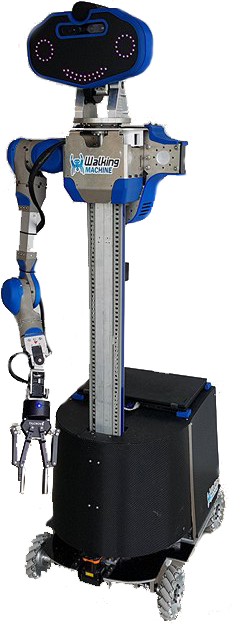
\includegraphics[width=0.30\textwidth]{images/sara_2.png}
	\caption{Robot SARA}
\end{wrapfigure}
\section*{Description logicielle du robot}



\begin{itemize}
	\item Plateforme: Robotic Operating System (ROS) Kinetic sur Ubuntu 16.04
	\item Navigation, localisation et construction de la map: \href{http://wiki.ros.org/gmapping}{Gmapping}, \href{http://wiki.ros.org/amcl}{AMCL}, \href{http://wiki.ros.org/pointcloud_to_laserscan}{pointcloud\_to\_laserscan}
	\item Reconnaissance faciale: \href{http://wiki.ros.org/people}{People}
	\item Reconnaissance vocale: \href{https://github.com/WalkingMachine/lab_ros_speech_to_text}{Google Speech API}
	\item Sémantique vocale: \href{http://sag.art.uniroma2.it/lu4r.html}{LU4R}, \href{https://github.com/WalkingMachine/lu4r_ros}{lu4r\_ros}
	\item Génération de la voix: \href{https://doc.ubuntu-fr.org/svoxpico}{Svoxpico}
	\item Reconnaissance d'objets: \href{https://github.com/WalkingMachine/wm_darknet}{Darknet with YOLO v2 }
	\item Contrôle du bras: \href{http://wiki.ros.org/moveit}{MoveIt} and \href{https://github.com/Kinovarobotics/kinova-ros}{Kinova API}
	\item Exécution des tâches: \href{http://wiki.ros.org/flexbe}{Flexbe} 
	\item Représentation de l'environnement: \href{http://github.com/walkingmachine/wonderland}{Wonderland}
\end{itemize}